\chapter{Experience Cannot Be Googled}

This interview segment is short, but its structure is exact. The question is not simply whether sales is useful. The question is how the skills learned in sales can become part of the machinery of company ownership. The answer does not begin with finance, hiring, legal structure, or strategy. It begins with something more primitive: repeated contact with resistance, and the ability to keep delivering a message after that resistance has arrived.

\section{From Salesman To Company Owner}

The opening question asks how the skills learned from being a salesman translated into owning a company at a young age. That is the local puzzle of the passage. A listener might expect an answer about closing techniques, networking, capital, or confidence. The speaker instead gives a more basic answer: experience is not something one can search for and possess.

\subsection{Question \& Answer}

\paragraph{Question.}
How do sales skills help someone become a company owner?

\paragraph{Answer.}
They help because sales forces a person through live commercial pressure. Scripts, appearance, and advice may prepare the surface, but the deeper skill comes from being rejected repeatedly and still delivering the message in the right way.

The point is not that sales automatically creates an owner. The point is narrower and more useful: sales trains the behavior that ownership later requires. A company owner must communicate, absorb refusal, adjust without collapsing, and continue representing the offer clearly. Sales gives that training in a concentrated form.

\section{Experience Versus Information}

The first claim is repeated for emphasis: experience cannot be Googled. The speaker is distinguishing information from exposure. Information can be copied, watched, searched, and repeated. Experience must be passed through.

\begin{remark}
In these notes, ``experience'' should not be inflated into a vague inspirational word. In this passage it means lived sales exposure: cold calls, door knocking, rejection, anger from prospects, and conversations with many kinds of people.
\end{remark}

That distinction matters for entrepreneurship because owning a company is not only a problem of knowing what to say. It is a problem of saying it under conditions that are not arranged for our comfort. The market does not merely ask whether the pitch is polished. It tests whether the person can keep functioning when the answer is no.

\section{Surface Preparation And Field Skill}

The speaker does not deny that a person can be taught. Someone can teach tricks, lines, useful things to say, and even how to dress. Those things belong to surface preparation. They are real, but incomplete.

\begin{table}
\centering
\begin{tabular}{p{0.42\linewidth}p{0.42\linewidth}}
\hline
Surface preparation & Field-tested skill \\
\hline
Things to say & Saying them after rejection \\
Polished dress & Maintaining composure under pressure \\
Sales tricks & Reading different people in real time \\
Instruction & Repeated commercial exposure \\
\hline
\end{tabular}
\caption{The transcript contrasts teachable preparation with the live pressure that turns preparation into usable sales skill.}
\end{table}

The rhythm here is important. The answer first grants the value of preparation, then immediately limits it. Until the person has been told no, cussed out, screamed at, and refused again and again, the technique has not yet been tested in the environment where it must work.

\section{Rejection As The Training Medium}

The emotional center of the passage is the repeated no. The speaker does not describe rejection as a single discouraging event. He describes it as a sequence: no after no after no. The educational medium is repetition under pressure.

This is why the chapter should not reduce the lesson to ``be resilient.'' Resilience is part of it, but the transcript is more specific. The skill is to receive rejection and still preserve the quality of the message.

\begin{definition}
Rejection pressure is the repeated experience of refusal, anger, or dismissal from prospects while the salesperson remains responsible for delivering the message clearly.
\end{definition}

The mechanism is practical. If every refusal changes the salesperson's attitude, tone, or clarity, the message deteriorates. Sales becomes a training ground because it exposes that deterioration quickly. The person either learns to recover, or the next call suffers.

\section{Delivering The Message The Right Way}

The key phrase is that one must still have the same attitude and still be able to deliver the message the right way. This is the hinge of the passage. The speaker is not merely saying that rejection is unpleasant. He is saying that rejection creates the condition under which real sales ability is measured.

\begin{figure}
\centering
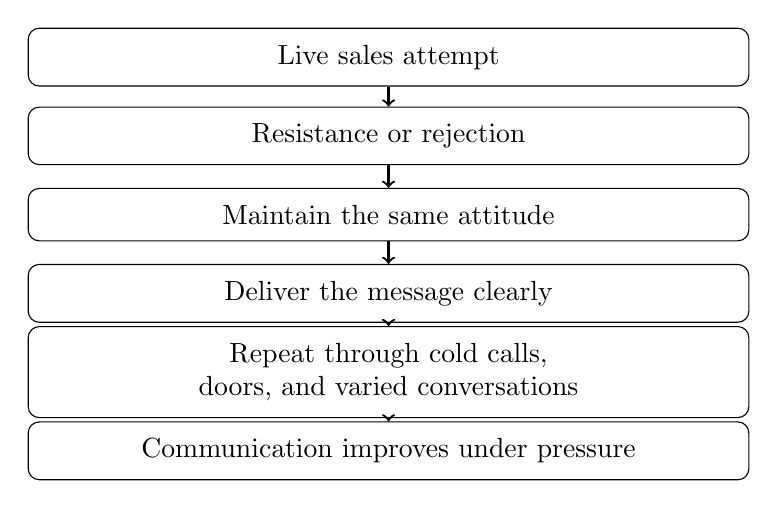
\begin{tikzpicture}[
  node distance=0.65cm,
  every node/.style={
    draw,
    rounded corners,
    align=center,
    text width=0.72\linewidth,
    inner sep=6pt
  },
  arrow/.style={->, thick}
]
\node (a) {Live sales attempt};
\node (b) [below of=a, yshift=-0.35cm] {Resistance or rejection};
\node (c) [below of=b, yshift=-0.35cm] {Maintain the same attitude};
\node (d) [below of=c, yshift=-0.35cm] {Deliver the message clearly};
\node (e) [below of=d, yshift=-0.35cm] {Repeat through cold calls, doors, and varied conversations};
\node (f) [below of=e, yshift=-0.35cm] {Communication improves under pressure};

\draw[arrow] (a) -- (b);
\draw[arrow] (b) -- (c);
\draw[arrow] (c) -- (d);
\draw[arrow] (d) -- (e);
\draw[arrow] (e) -- (f);
\end{tikzpicture}
\caption{A transcript-derived process view of the speaker's mechanism: repeated sales exposure turns rejection into communication practice.}
\end{figure}

This figure is not presented as an on-screen diagram. It is a compact reconstruction of the spoken sequence. The order matters: attempt, resistance, attitude, message, repetition, improvement.

\section{Thousands Of Repetitions}

The speaker then returns to the earlier point in a new form. There is no textbook that can teach this, he says, apart from making thousands and thousands of cold calls, knocking on doors, and passing through many different experiences.

The phrase ``thousands and thousands'' should be kept as a qualitative magnitude. It is not a measured statistic in the transcript. Its force is that sales skill is accumulated through volume. The same act is repeated, but each repetition arrives with a different person, mood, objection, and outcome.

\begin{remark}
The claim is not that books, scripts, or coaching have no value. The claim is that they cannot substitute for the number of live encounters required to make the behavior durable.
\end{remark}

This is where the passage begins to connect directly to ownership. A company owner faces markets, partners, employees, customers, vendors, and investors. Not all of those conversations are sales calls, but many of them require the same underlying behavior: communicate clearly when the other side is not giving easy approval.

\section{Communication Across Difference}

The final movement widens the lesson. Sales teaches communication across different ethnicities, backgrounds, ages, and experiences. The speaker's argument is not only that rejection makes a person tougher. It is also that repeated selling makes a person more flexible.

A single social environment can reward a narrow style of communication. Sales punishes narrowness. The salesperson has to find a way to speak with people who do not share the same background, expectations, patience, or frame of reference. That variety becomes part of the education.

\begin{proposition}
In the speaker's account, sales contributes to company ownership by training adaptable communication under repeated rejection and social variety.
\end{proposition}

\begin{proof}
The transcript gives the sequence directly. First, the speaker says experience cannot be searched for or learned only from instruction. Second, he identifies repeated rejection as the condition that tests the salesperson. Third, he says the salesperson must maintain attitude and deliver the message properly despite that rejection. Fourth, he grounds the learning in thousands of cold calls, door knocking, and many experiences. Finally, he broadens the setting to communication with people across different backgrounds, ages, and experiences. Together these claims support the narrower proposition: sales trains communication that remains usable under pressure and across difference.
\end{proof}

\section{Summary}

The passage answers a practical entrepreneurial question by refusing the shortcut. Sales helped because it supplied experience that could not be Googled: rejection, repetition, door knocking, cold calls, and conversations with many kinds of people. The useful skill was not merely knowing what to say. It was keeping the same attitude and delivering the message correctly after resistance. That is why, in this interview, sales becomes a bridge to ownership: it trains the person to communicate clearly when the market is not cooperating.